\newpage
% \label{sec:app_integrator}
\hypertarget{sec:app_integrator}{}
\section{Using the Integrator}
\genHeader

Let's check out another cool visualization feature of eMoflon, the integrator. The graph viewer allows you to ``see" the structure of a model, but the
integrator allows you to actually trace the transformation process. In other words, the integrator works as an ``offline'' debugger.

\begin{itemize}

\item[$\blacktriangleright$] Right-click on \texttt{corr\_BWD.xmi} and choose ``eMoflon/Start Integrator'' which will open the window depicted in
Fig.~\ref{eclipse:integrator_start}. This first window depicts your TGG triple, showing how the \texttt{source} and \texttt{target} metamodels are connected
via the \texttt{link} (correspondence) metamodel.

\begin{figure}[htbp]
\begin{center}
  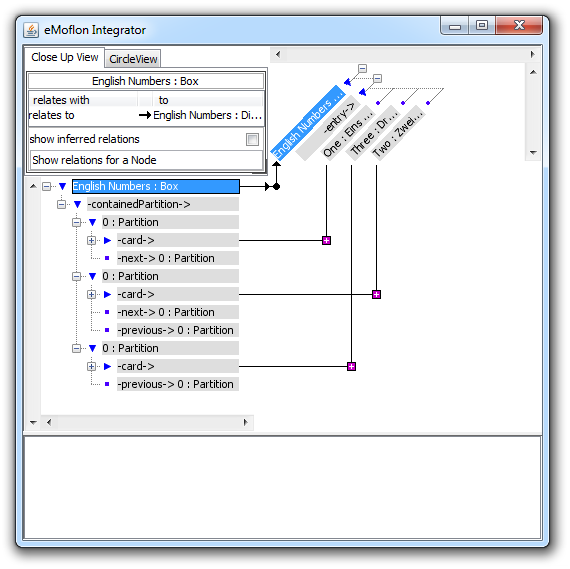
\includegraphics[width=0.7\textwidth]{eclipse_integratorStart}
  \caption{Default view of the integrator}
  \label{eclipse:integrator_start}
\end{center}
\end{figure}

\item[$\blacktriangleright$] Drag and drop \texttt{protocol\_BWD.xmi} into the main window.\footnote{If the integrator window minimizes, press \texttt{alt+tab}
to re-activate it} You will be able to see the controls for navigating through the transformation process explained in the lower part of the window.

\item[$\blacktriangleright$]  Use \texttt{Alt+Right} to navigate forwards through the transformation, and \texttt{Alt+Left} to go backwards. A brief description
of each step will appear in the small window below.

\item[$\blacktriangleright$] As you progress through the transformation, the window will state what node is currently active, and list the possible actions
(rule candidates) that may be applied to that object. 

\vspace{0.5cm}

\begin{figure}[h!]
\begin{center}
  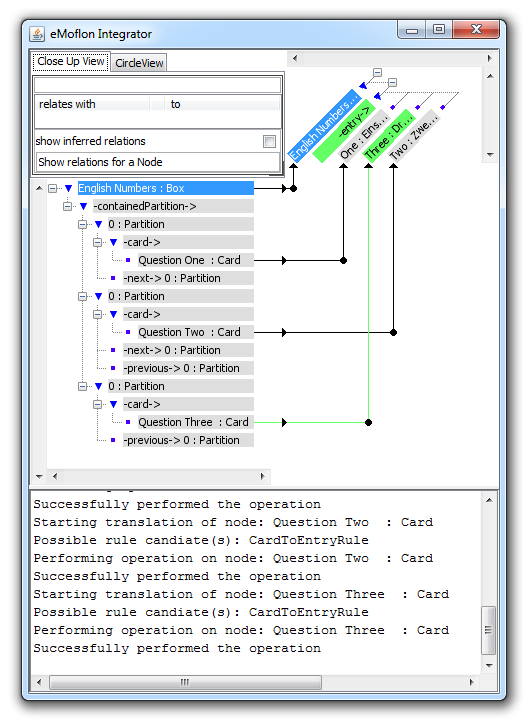
\includegraphics[width=0.55\textwidth]{eclipse_integratorPerformed}
  \caption{Integrator after the complete process}
  \label{eclipse:integrator_after_protocol}
\end{center}
\end{figure} 

\item[$\blacktriangleright$] While stepping through the transformation, you'll notice there are colours for each node based on their state. They represent how
the element is currently being processed, and are defined as follows:

\begin{description}
  \item[Blue] The element is currently being ``looked at," and is about to be processed.

  \item[Yellow] The element cannot be transformed right now and has been queued for later transformation (i.e., when transforming the first
  \texttt{Entry} into a \texttt{Card}, the \texttt{Box} with the \texttt{partition} to store \texttt{card} must be translated first); ``Pending.''
  
  \item[Green] The object has been created.

\end{description}

\end{itemize}
